\section{NAX分析}
\subsection{发行量分析}
由于每期增发池中未发放的部分滚入下一期增发池中,因此总发行量为固定值,可以因此推导出初始的预增发量,如果我们将总发行量设定为100亿(\(10^{10}\)),那么可以推导出第0期预发行的规模如下:
\begin{equation}
  \sum_{i,j} K_{i,j} = \sum_i C_0 \mu^i = \frac{C_0}{1-\mu}
\end{equation}
  令此上界为100亿(\(10^{10}\)),可解出\(C_0 = 10^{10}(1-\mu) = 1.0\times10^7\)。

\subsection{发放比例与质押率关系}
发放比例和质押率的关系,如图\ref{func}根据需求,发放比例的取值在0到1之间,例如,质押率为30\%时增发比例为70\%,质押率为50\%时增发比例为90\%。其中\(l=1.52\), \(m=-3.88\), \(n=3.36\)。

\subsection{权重与币龄的关系}
为了使得鼓励早期参与质押的用户,同时也不打击新进质押用户的积极性,我们设计的函数将使得早期用户相对新用户,在分发权重上有所不同,但随着周期数的上升,当质押到达90个周期后,权重将趋于平稳,比如到达$1$。为了鼓励新用户也争相加入质押,新用户的权重也不是完全从0开始,起始的权重将从一个基础开始,比如说:$0.67$. 因此,根据上述方程\ref{func}所示,我们可以得出相应的系数,其中\(a=0.005\),\(b=-0.3\),\(c=0.2\),该函数如图\ref{weight}所示。可见有效权重的值在0.67到1之间,随质押周期数的增加而不断接近1,质押周期数为30(约1个月)时有效权重为0.8,质押周期数为60(约2个月)时有效权重为0.9,质押周期数为90(约3个月)时有效权重为0.95。

\subsection{币龄对收益的影响}
在质押数量相同的情况下,起始质押时间所产生的币龄将对收益产生的影响。 这个影响的大小并不是非常的明显,下面我们给出一个我们模拟出来的一个效果作为示例,如图\ref{fig:compare}所示, 注:该图只作比较性参考,不反应实际收益情况,实际收益多少也和整体质押数量和地址有关。
\begin{figure}[htbp]
  \centering
    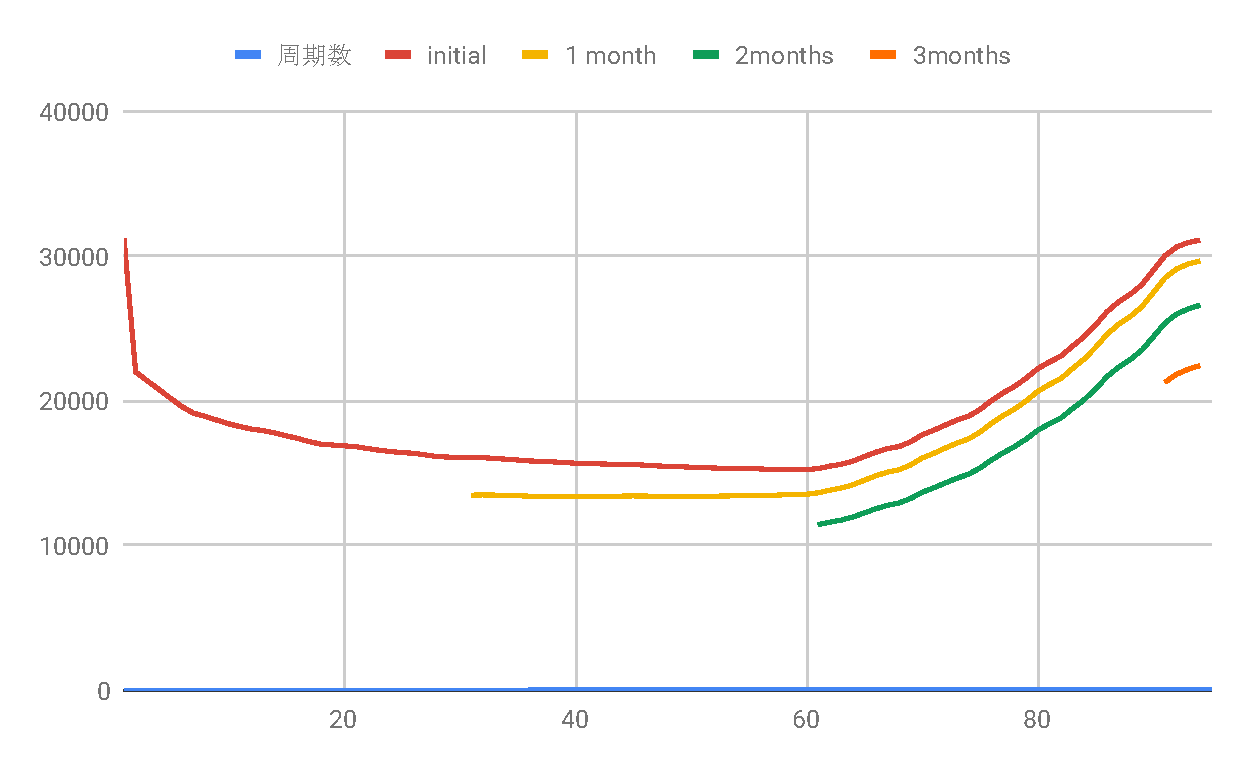
\includegraphics[width=0.6\textwidth]{../common/compare.pdf}
    \caption{质押起始时间对收益的影响 \label{fig:compare}}
\end{figure}

\subsection{追加质押对币龄的影响 -- 平均币龄}
为了便于用户在原地址基础上追加更多的质押,用户只需要对质押合约地址做一次$0$ NAS交易,或者调用质押合约相应的接口,达到更新质押契约的目的。系统会根据过去质押和新质押的数量,重新计算出新的质押币龄。例如,用户当前质押$100$NAS, 币龄是$10$个周期,这个时候用户追加另外$100$ NAS,并通知质押合约这$100$ NAS全部进入新的质押。那么现在质押数量变成了$200$ NAS,而币龄则变成两次质押的平均币龄了$5$个周期。